\chapter{Filtros}

Un filtro, sea activo o pasivo (que no contiene amplificadores), permiten que cierta porción del espectro de frecuencias pase por su salida. El filtro se clasifica de acuerdo con la porción del espectro de frecuencias que deja pasar.

Los filtros paso-bajos dejan pasar frecuencias desde cero hasta alguna frecuencia de corte seleccionada, $f_c$, y atenúan todas las frecuencias superiores a $f_c$. A la gama de frecuencias de cero a $f_c$ se le llama banda de paso. A la gama de frecuencias superiores a $f_b$ se le llama banda de bloqueo. A la gama de frecuencias de $f_c$ a $f_b$ se le llama región de transición. La proporción en que varía la atenuación en la región de transición es una característica importante del filtro. La frecuencia a la cual el voltaje de salida del filtro cae a un valor de 0.707 de su valor en la banda de paso (o sea, que ha disminuido en 3 dB) es la frecuencia de corte, $f_c$. La frecuencia a la cual el voltaje de salida está 3 dB arriba del valor en la banda de bloqueo es $f_b$.

El filtro paso-altos atenúa todas las frecuencias hasta $f_c$ y deja pasar todas las frecuencias superiores a $f_c$ hasta el límite de frecuencia del filtro paso-altos.

Un filtro paso-banda deja pasar todas las frecuencias entre una frecuencia inferior de corte, $f_1$, y una frecuencia superior de corte, $f_2$. Todas las frecuencias inferiores a $f_1$ y superiores a $f_2$ son atenuadas. Las gamas de frecuencias de $f'_1$ a $f_1$ y de $f_2$ a $f`_2$ son las regiones de transición. La frecuencia central $f_0$ se considera como la media geométrica de $f_1$ y $f_2$ y se encuentra a partir de esta ecuación:

\begin{equation}
    f_0 = \sqrt{f_1 f_2}
\end{equation}

\section{Ventajas de los filtros activos}
Las ventajas de los filtros activos respecto a los pasivos son las siguientes:
\begin{enumerate}
    \item Utilizan resistencias y condensadores que se comportan más idealmente que los inductores.
    \item Son relativamente baratos.
    \item Pueden dar ganancia en la banda de paso y rara vez tienen pérdidas severas (como las tienen los filtros pasivos).
    \item El empleo de amp-ops en los filtros activos proporciona separación entre la entrada y la salida. Esto permite que los filtros activos puedan conectarse fácilmente en cascada a fin de obtener un mejor funcionamiento.
    \item Los filtros activos son relativamente fáciles de alinear.
    \item Se pueden construir filtros de muy baja frecuencia usando componentes de poco valor.
    \item Los filtros activos son pequeños y ligeros.
\end{enumerate}

Los filtros activos tienen desventajas. Requieren una fuente de alimentación y su frecuencia máxima está limitada a la frecuencia más alta de operación del amp-op.

\section{Tipos de respuesta del filtro}
\subsection{Butterworth}
La respuesta de un filtro Butterworth (Figura \ref{fig:Butterworth}) es muy plana en la banda de paso. Se dice que su respuesta es máximamente plana. La variación de atenuación de un filtro Butterworth en la región de transición es de 20dB/década por cada polo. La respuesta de fase de un filtro Butterworth no es lineal. Dicho de otro modo, el tiempo necesario para que una señal se propague a través del filtro no es lineal con la frecuencia. Por tanto una respuesta de escalón o pulso aplicado a un filtro Butterworth provocará un exceso en la salida. Este filtro se usa cuando todas las frecuencias de la banda de paso deben tener la misma ganancia.

\begin{figure}[H]
    \centering
    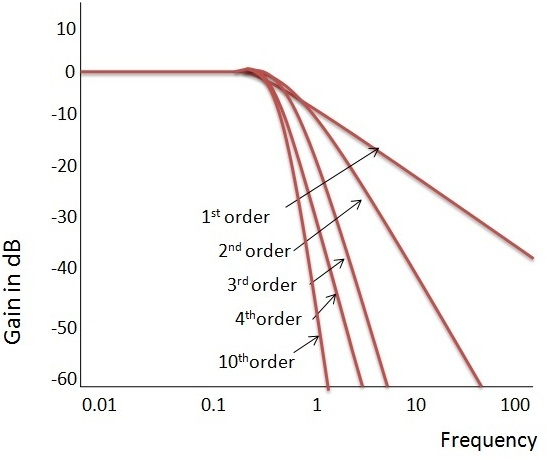
\includegraphics[width=0.5\linewidth]{Imagenes/Filtros Butterworth.png}
    \caption{Curva de respuesta del filtro Butterworth.}
    \label{fig:Butterworth}
\end{figure}

\subsection{Chebychev}
Un filtro Chebyshev tendrá ondulaciones en la banda de paso, pero no en la banda de bloqueo. Mientras más alto sea el orden del filtro, más ondulaciones aparecerán en la banda de paso. La amplitud de la ondulación puede establecerse en el filtro al diseñarlo y casualmente se fija a 0.5 dB, 1 dB, 2 dB ó 3 dB. Mientras más ondulación se permita, más atenuación se obtendrá en la región de transición.

\begin{figure}[H]
    \centering
    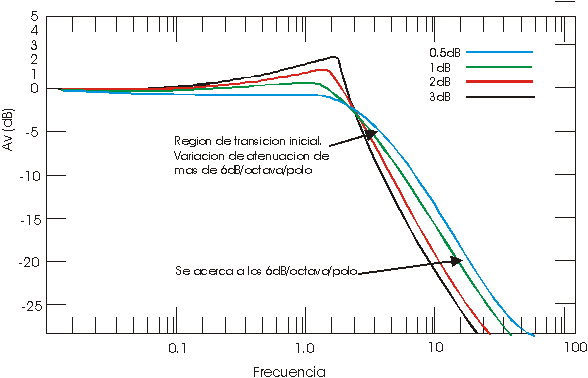
\includegraphics[width=0.5\linewidth]{Imagenes/Filtros Chebyshev.png}
    \caption{Curva de respuesta del filtro Chebyshev.}
    \label{fig:Chebyshev}
\end{figure}

\subsection{Bessel}
A los filtros Bessel se les llama filtros de fase lineal o de retraso lineal en el tiempo. El retraso de fase de una señal, de la entrada a la salida, aumenta linealmente con la frecuencia. Por tanto, los filtros Bessel casi no tienen exceso con una entrada de respuesta en escalón. Esta característica hace que sean los mejores para filtras ondas rectangulares sin alterar la forma de la onda.. 

Los filtros Bessel tienen una variación de atenuación en la región de menos de 20 dB/década. La frecuencia de corte del Bessel se define como la frecuencia a la cual el retraso de fase del filtro es la mitad del retraso de fase máximo. La frecuencia de 3 dB de un filtro Bessel no es la $f_c$ definida.

\begin{figure}[H]
    \centering
    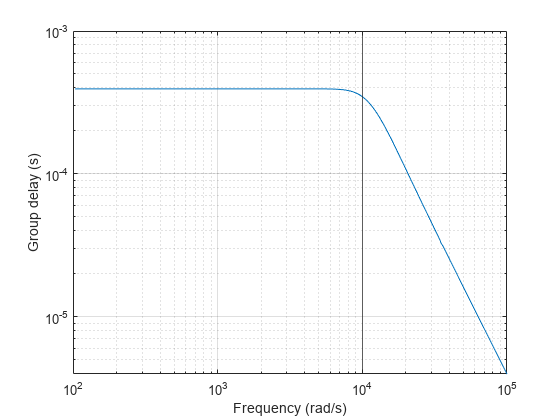
\includegraphics[width=0.5\linewidth]{Imagenes/Filtros Bessel.png}
    \caption{Curva de respuesta del filtro Bessel.}
    \label{fig:Bessel}
\end{figure}

\section{Algunas definiciones}

El factor de amortiguación, $\alpha$, determina la forma de la región de transición y el exceso de la respuesta de banda de paso cerca de la región de transición. Por tanto determina la forma de la respuesta del filtro y el tipo de filtro. Un filtro Bessel, un Butterworth y un Chebyshev podrían tener el mismo diagrama, que sólo diferirá en los valores de los componentes.

\begin{figure}[H]
    \centering
    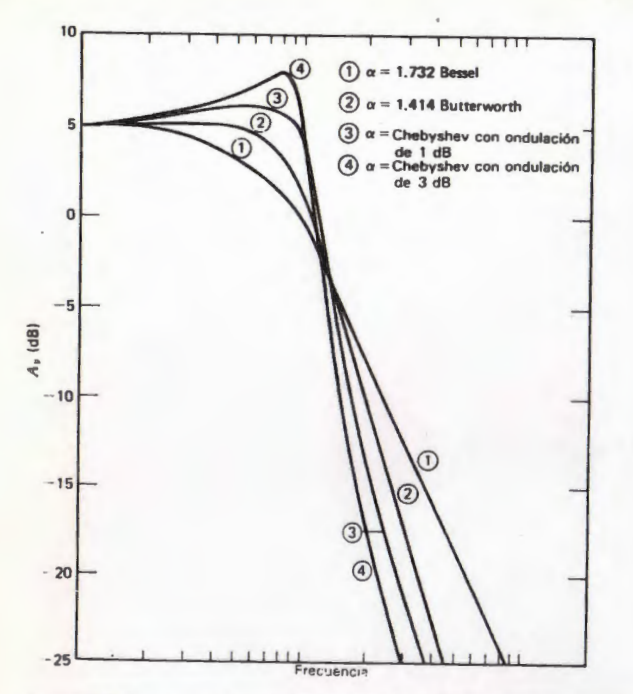
\includegraphics[width=0.5\linewidth]{Imagenes/Filtros Factor de Amortiguacion.png}
    \caption{Respuestas de paso-bajas variando el factor de amortiguación.}
\end{figure}

El factor de calidad, $Q$, es la relación entre la frecuencia central de paso-banda y las frecuencias de 3 dB en un circuito paso-banda.

\begin{equation}
    Q = \frac{f_0}{f_2 - f_1} = \frac{\sqrt{f_1 f_2}}{f_2 - f_1}
\end{equation}

donde 
\begin{itemize}
    \item $f_0 = \sqrt{f_1 f_2} = $ frecuencia central
    \item $f_1 = $ frecuencia inferior de 3dB
    \item $f_2 = $ frecuencia superior de 3dB
\end{itemize}

En el caso de los filtros activos,

\begin{equation}
    Q \approx \frac{1}{\alpha}
\end{equation}

La ganancia del filtro activo en su banda de paso es la ganancia de banda de paso.

\begin{equation}
    A_p \approx \frac{V_{sal}}{V_{ent}}
\end{equation}

La sensibilidad, $S$, es la proporción en que varía un parámetro del filtro conforme se varía otro parámetro.

\section{Algunos tipos de filtros activos}
\subsection{El Sallen y Key (VCVS)}
VCVS son las siglas en inglés de fuente de voltaje controlada por voltaje. En estos circuitos, el amp-op se usa como VCVS. Como hay dos circuitos $RC$, $R_1 C_1$ y $R_2 C_2$, los circuitos que se muestran son de segundo orden. En el circuito de paso-bajas, $R_1C_1$ y $R_2C_2$ son integradores. En el circuito de paso-altas, $R_1C_1$ y $R_2C_2$ son diferenciadores. $R_A$ y $R_B$ determinan el factor de amortiguación.

\begin{figure}[H]
    \centering
    \begin{subfigure}[c]{0.45\textwidth}
        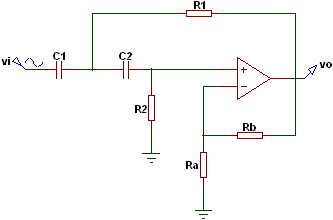
\includegraphics[width=\textwidth]{Imagenes/Filtros Sallen y Key Paso-Altas.png}
        \caption{Filtro paso-altas de segundo orden.}
    \end{subfigure}
    \begin{subfigure}[c]{0.45\textwidth}
        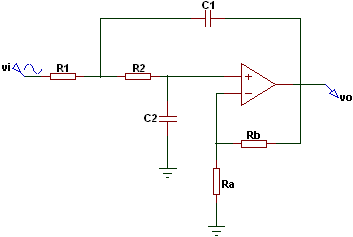
\includegraphics[width=\textwidth]{Imagenes/Filtros Sallen y Key Paso-Bajas.png}
        \caption{Filtro paso-bajas de segundo orden.}
    \end{subfigure}
\end{figure}

\subsection{De retroalimentación múltiple}
El filtro activo de retroalimentación múltiple es un filtro paso de banda, sencillo y de buen funcionamiento, para $Qs$ de bajos a moderados, hasta de 10 aproximadamente. Este circuito se muestra en la figura ---. Se observa como la retroalimentación tiene lugar a través de $C_1$ y de $R_3$. $R_1$ y $C_1$ proporcionan la respuesta paso-bajas y $R_3$ y $C_2$ proporcionan la respuesta paso-altas. La retroalimentación proporciona la maximización ($Q$) cerca de $f_0$. $R_2$ se puede omitir; pero se modifica el procedimiento de cálculo de los componentes. $R-2$ eleva la $R_{ent}$ y ofrece una ganancia controlable de banda de paso.

\begin{figure}[H]
    \centering
    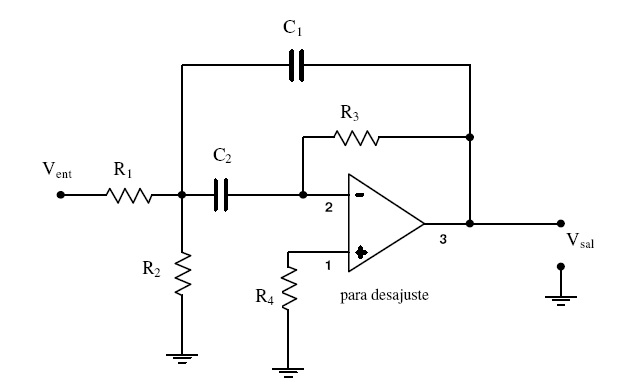
\includegraphics[width=0.5\linewidth]{Imagenes/Filtros de Retroalimentacion Multiple.png}
    \caption{Filtros paso-banda de retroalimentación múltiple.}
\end{figure}

\subsection{De variable de estado}
El filtro de variable de estado es muy estable, tienen bajas sensibilidades $Q$ y $\alpha$ y hay poca interacción entre los ajustes de frecuencia y el $Q$. Si se usa como filtro paso-banda se pueden obtener $Qs$ estables hasta de 100. El filtro con variable de estado, llamado a veces ``filtro activo universal'', se usa en muchos filtros activos comerciales.

\subsection{El bicuadrático (Bicuad)}
El filtro bicuadrático (bicuad) es un filtro activo muy estable, fácil de conectar en cascada, capaz de dar $Qs$ de más de 100 en la aplicación paso-banda. Una de las características del bicuad es que su ancho de banda permanece constante a medida que se varía su frecuencia, de manera que su $Q$ aumenta con la frecuencia en los filtros ajustables. 

\begin{figure}[H]
    \centering
    \begin{subfigure}[c]{0.45\textwidth}
        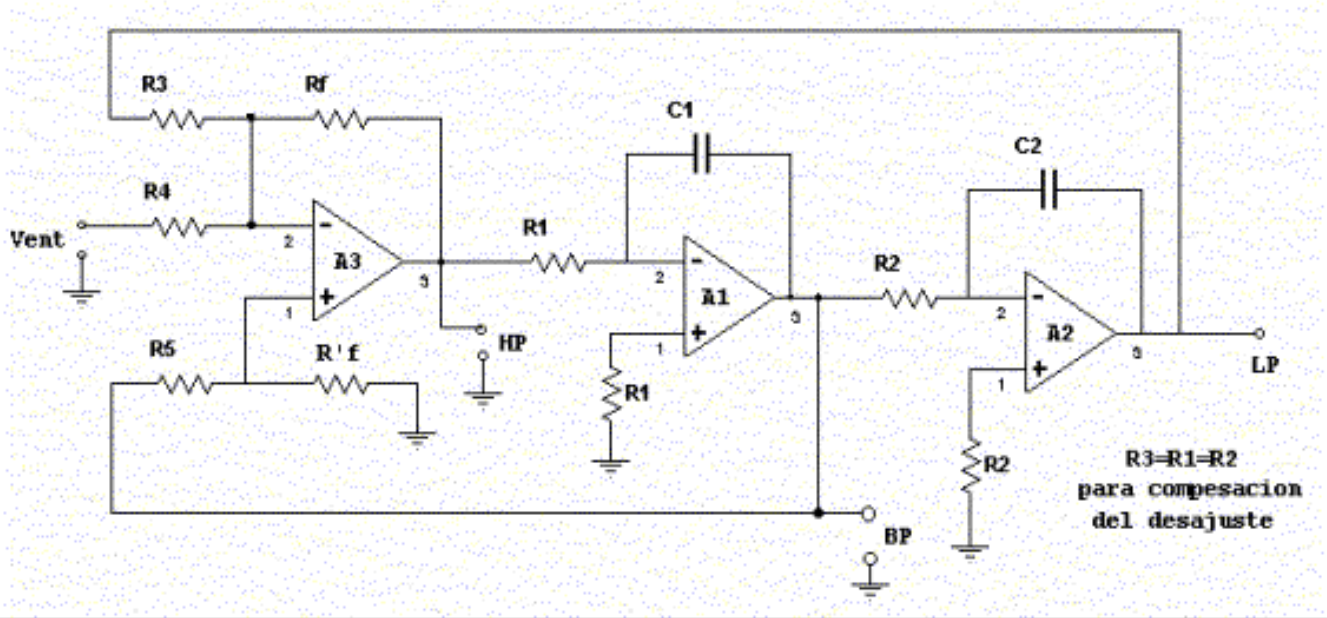
\includegraphics[width=\textwidth]{Imagenes/Filtros de Variable de Estado.png}
        \caption{Filtros de Variable de Estado.}
    \end{subfigure}
    \begin{subfigure}[c]{0.45\textwidth}
        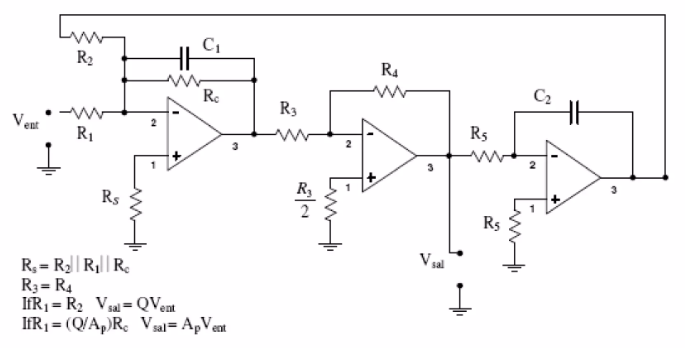
\includegraphics[width=\textwidth]{Imagenes/Filtros Bicuadratico.png}
        \caption{Filtro bicuadrático paso-banda.}
    \end{subfigure}
\end{figure}